% Final report: business entity resolution.
% Build:  cd report/latex && tectonic main.tex      (XeTeX; needs the macOS Sangam MN fonts for the
% few Devanagari / Malayalam examples)
% One file per section in sections/; the comment at the top of each file names its author.
\documentclass[11pt,a4paper]{article}

\usepackage[margin=2.4cm]{geometry}
\usepackage{fontspec}
\usepackage{microtype}
\usepackage{amsmath,amssymb}
\usepackage{booktabs,tabularx,multirow}
\usepackage{graphicx}
\usepackage[font=small,labelfont=bf]{caption}
\usepackage{xcolor}
\usepackage{tikz}
\usetikzlibrary{positioning,arrows.meta,fit}
\usepackage[hidelinks]{hyperref}
\usepackage[inline]{enumitem}
\setlist{nosep,leftmargin=*}

\newfontfamily\deva[Script=Devanagari]{Devanagari Sangam MN}
\newfontfamily\mlym[Script=Malayalam]{Malayalam Sangam MN}

\graphicspath{{../../analysis/out_gbm/}{../../analysis/out_rnn/}{../../analysis/out_script/}{../../}}

\newcommand{\fhalf}{F$_{0.5}$}
\newcommand{\nb}[1]{\texttt{#1}}          % notebook id, e.g. \nb{04}
\renewcommand{\arraystretch}{1.1}
\setlength{\tabcolsep}{4.5pt}

\title{Multilingual Business Entity Resolution:\\
Retrieval, Classical, Recurrent and Transformer Matchers\\ and a Gated Mixture of Experts}
\author{Akshat Gupta \and Keshav Mishra \and Rishi Kharya \and Shivam Singh \and Ayush Khelwal}
\date{NLP course project, November 2026}

\begin{document}
\maketitle

% Author: Keshav
\section{Introduction}
\label{sec:intro}

Entity resolution decides which records in different databases describe the same real-world
entity. Our task comes from the Amazon ML Challenge 2026: Source~1
(S1) is a reference list of businesses, and every record of Sources~2 and~3 (S2, S3) has to be linked to the
S1 entity it describes, or to none. The data covers the US and India. The noise is varied:
\begin{itemize}
  \item abbreviated legal forms (\emph{private limited} / \emph{pvt ltd});
  \item phonetic romanisations of Indian words (\emph{praivtt}, \emph{enjiniyring});
  \item names written in Devanagari or Malayalam, while S1 is always in Latin script;
  \item missing addresses;
  \item near-duplicate branches of one chain that differ only in a house number.
\end{itemize}
About a quarter of S2/S3 records have no S1 entity at all. The metric is macro \fhalf{} per S1 entity,
which weighs precision more than recall, so a wrong link costs more than a missed one.

This makes the task a good test bed for the course material. It needs tokenization that copes with
three scripts, string similarity and edit distance, sequence labelling (address parsing), recurrent
networks, pre-trained transformers with full and parameter-efficient fine-tuning, and Mixture-of-Experts
models. We built one shared pipeline (\S\ref{sec:overview}) in which every matcher scores \emph{the same}
candidate pairs with \emph{the same} decision rule and threshold protocol, so that their results are
directly comparable. The sections below follow the pipeline: data and splits (\S\ref{sec:data}), tokenization and retrieval (\S\ref{sec:tok}), parsing, the classical, recurrent and transformer matchers including Ditto (\S\ref{sec:parsing}--\ref{sec:ce}), Mixture-of-Experts fusion (\S\ref{sec:fusion}) and a per-script error analysis (\S\ref{sec:script}).
Table~\ref{tab:main} in \S\ref{sec:fusion} collects all results.

% Author: Keshav
\section{Related work}
\label{sec:related}

\paragraph{Record linkage.} Fellegi and Sunter formalised record linkage as classifying record
pairs from field agreement patterns. Since comparing all pairs is quadratic, practical systems first
\emph{block}, i.e.\ generate a small candidate set per record, and then \emph{match}
candidates. Classical matchers compare fields with string
similarities such as edit distance and Jaro--Winkler.
We follow the block-then-match design and use these similarities as features of a gradient-boosted
classifier.

\paragraph{Deep entity matching.} DeepMatcher compared RNN- and attention-based
attribute summarisers for matching. Ditto cast matching as sequence-pair classification
with a fine-tuned pre-trained language model and added domain-knowledge injection, summarisation and data
augmentation. We reproduce Ditto's ablation on our data. Our Siamese recurrent
matchers follow Mueller and Thyagarajan, with LSTM and GRU
cells. We measure the vanishing-gradient problem that
separates them from a vanilla RNN.

\paragraph{Retrieval and reranking.} Our two-stage design mirrors open-domain QA: a bi-encoder retriever
trained with in-batch negatives, here multilingual-e5,
followed by a cross-encoder reranker, here bge-reranker.
Sparse and dense lists are merged with reciprocal rank fusion.

\paragraph{Multilingual and Indic models.} We compare multilingual encoders (mBERT,
XLM-R, mDeBERTa-v3) with the Indic-specific
IndicBERTv2, and measure tokenizer fertility as in Rust et al..
Parameter-efficient fine-tuning uses LoRA.

\paragraph{Address parsing.} Neural sequence labelling with a BiLSTM and a CRF output
layer is the standard model for address
parsing. We have no gold parses, so we train on silver labels from rules, a
form of weak supervision.

\paragraph{Mixtures of experts and stacking.} A mixture of experts weights expert outputs with an
input-dependent gate; sparse top-$k$ gates with a load-balancing loss scale this
idea to large networks. We use both forms: a top-2 MoE head
inside a cross-encoder, and a dense gate over whole matchers. We compare the latter with stacked
generalisation.

% Author: Akshat (condensed from report/section_data_tokenization_retrieval.md, part D)
\section{Data, splits and metric}
\label{sec:data}

\paragraph{Task and decision rule.} Each S2/S3 record is linked to at most one S1 entity; 26\% are linked to
none. Every model uses the same \textbf{decision rule}: a record is assigned to its best-scoring S1 candidate
if the score reaches a threshold $\tau$, and to no S1 otherwise. This is the mention-ranking formulation of
coreference with a dummy antecedent: each record either picks its best antecedent or
starts a new cluster.

\paragraph{Metric.} For every S1 entity we compare the set of S2/S3 records predicted for it with its true
set, compute \fhalf, and average over all S1 entities (macro \fhalf). Singletons, i.e.\ S1 entities with no
true match, are included and score 1 only if nothing is linked to them. Our implementation scores 1.0 on the
ground truth, 0.05585 on an empty prediction (the singleton share), and 0.87114 when the last true record of
every S1 entity is dropped (P 1.0, R 0.66).

\paragraph{Splits.} The official test set has no labels, so all results come from splits of the labelled
training data. The unit is the \textbf{S1 entity}, split 70/10/20 into train/val/test; linked S2/S3 records
follow their S1, so no business is seen in both training and test. Splits are stratified by country $\times$
number of true matches (0 / 1--3 / 4+). Unlinked S2/S3 records (distractors) are spread in the same
proportions by a hash of their id, which keeps the distractor density of the original data. All random
choices use BLAKE2b hashes. We tried CRC32 first, but CRC hashes of one id under different seeds are
correlated.

\paragraph{Regional subset.} Training on the full data (2.2M S1 entities) is beyond free Kaggle T4 GPUs,
so we keep four \emph{whole} states: Oregon and Utah (US), Kerala and Madhya Pradesh (India). Whole states
keep a region's near-duplicate businesses together, so matching stays as hard as on the full data.
States are spelled differently in each source (\emph{TX}/\emph{Texas}). The split script learns the mapping
from address components to states from the ground-truth links: 81 canonical states, 15,095 spellings.
Table~\ref{tab:splits} gives the sizes.

\begin{table}[h]
\centering\small
\begin{tabular}{lrrrrrr}
\toprule
split & S1 (US / India) & singletons & true links & S2 & S3 & unlinked pool \\
\midrule
train & 75,353 (36,238 / 39,115) & 4,169 & 261,183 & 173,057 & 182,320 & 94,194 (26.5\%) \\
val   & 10,764 (5,176 / 5,588)    & 595   & 37,236  & 24,896  & 25,856  & 13,516 (26.6\%) \\
test  & 21,529 (10,353 / 11,176)  & 1,191 & 74,619  & 49,479  & 52,095  & 26,955 (26.5\%) \\
\bottomrule
\end{tabular}
\caption{Splits of the regional subset (\texttt{data/small}).}
\label{tab:splits}
\end{table}

\paragraph{Protocol.} Everything (models, TF-IDF vocabularies, the transliteration lexicon, normalisation
rules) is fitted on train. Hyper-parameters and thresholds are tuned on val. Test is scored once per final
model, and its labels are read only inside the final scoring function.

\paragraph{Limitations of the splits.} (i)~Our splits have about 1.2 unlinked records per S1 entity; on the
official test set we measured about 2.3 during the challenge. Our \fhalf{} is therefore optimistic, mostly in
precision. (ii)~The subset holds about 3.5\% of the S1 entities, so absolute numbers are not those of a
full-data model; the ranking of methods should carry over.

% Author: Keshav
\section{System overview}
\label{sec:overview}

\begin{figure}[t]
\centering
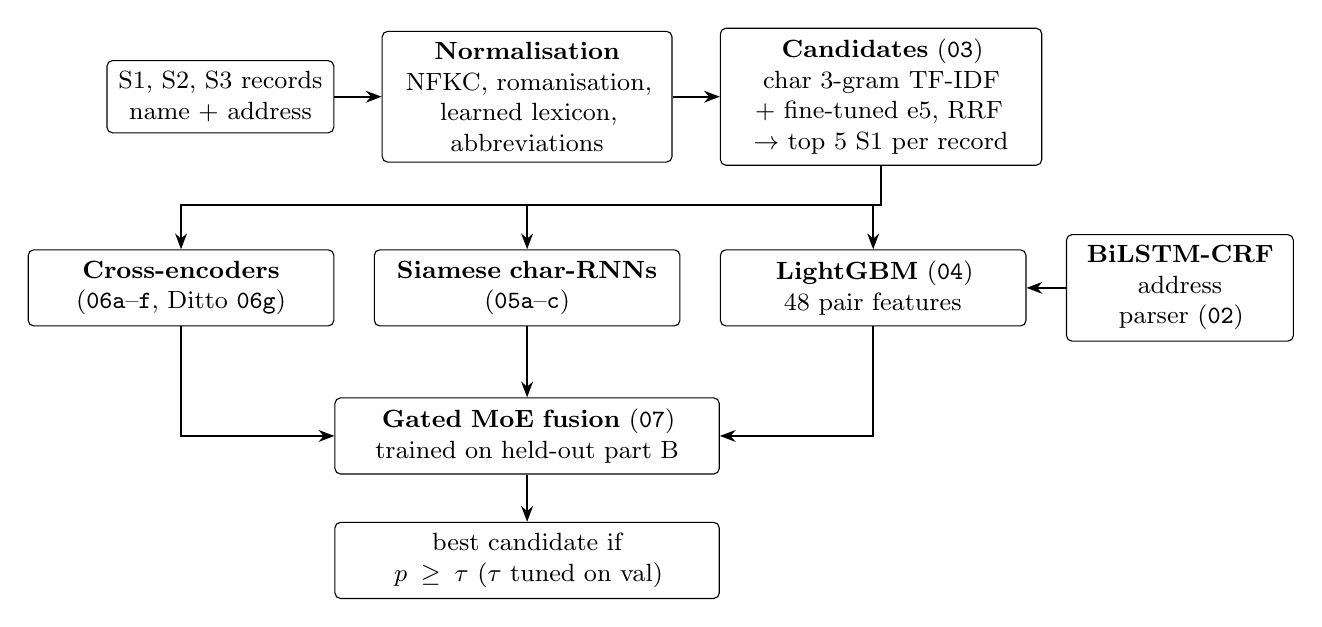
\begin{tikzpicture}[
  box/.style={draw, rounded corners=2pt, align=center, font=\small, inner sep=4pt, text width=#1},
  box/.default=3.4cm,
  arr/.style={-{Stealth[length=2mm]}, thick}]
\node[box=2.6cm] (raw) {S1, S2, S3 records\\ name + address};
\node[box, right=0.6cm of raw] (norm) {\textbf{Normalisation}\\ NFKC, romanisation,\\ learned lexicon,\\ abbreviations};
\node[box=3.8cm, right=0.6cm of norm] (cand) {\textbf{Candidates} (\nb{03})\\ char 3-gram TF-IDF\\ + fine-tuned e5, RRF\\ $\rightarrow$ top 5 S1 per record};
\node[box=3.6cm, below=1.1cm of norm] (m05) {\textbf{Siamese char-RNNs}\\ (\nb{05a}--\nb{c})};
\node[box=3.6cm, left=0.5cm of m05] (m06) {\textbf{Cross-encoders}\\ (\nb{06a}--\nb{f}, Ditto \nb{06g})};
\node[box=3.6cm, right=0.5cm of m05] (m04) {\textbf{LightGBM} (\nb{04})\\ 48 pair features};
\node[box=2.6cm, right=0.5cm of m04] (m02) {\textbf{BiLSTM-CRF}\\ address parser (\nb{02})};
\node[box=4.6cm, below=0.9cm of m05] (moe) {\textbf{Gated MoE fusion} (\nb{07})\\ trained on held-out part B};
\node[box=4.6cm, below=0.6cm of moe] (dec) {best candidate if $p \ge \tau$ ($\tau$ tuned on val)};
\draw[arr] (raw) -- (norm);
\draw[arr] (norm) -- (cand);
\draw[arr] (cand.south) -- ++(0,-0.5) -| (m04.north);
\draw[arr] (cand.south) -- ++(0,-0.5) -| (m05.north);
\draw[arr] (cand.south) -- ++(0,-0.5) -| (m06.north);
\draw[arr] (m02) -- (m04);
\draw[arr] (m06.south) |- (moe.west);
\draw[arr] (m05) -- (moe);
\draw[arr] (m04.south) |- (moe.east);
\draw[arr] (moe) -- (dec);
\end{tikzpicture}
\caption{Pipeline. Every matcher scores the same candidate pairs and saves logits; the fusion learns how
much to trust each matcher. Numbers in parentheses are the project notebooks.}
\label{fig:pipeline}
\end{figure}

Figure~\ref{fig:pipeline} shows the pipeline. It is implemented as a series of Kaggle notebooks generated
from one source file, so all of them share the data loading, normalisation and evaluation code.

\paragraph{Normalisation.} All text goes through one shared step: Unicode NFKC, romanisation of
non-Latin scripts, lower-casing, abbreviation expansion, and a transliteration lexicon of 316 words learned
from the training links (Section~\ref{sec:tok}). Matchers read three views of a record:
\begin{itemize}
  \item TF-IDF and the string features read the fully normalised text;
  \item the Siamese RNNs read the normalised \texttt{name | address}, cut at 100 characters;
  \item the e5 retriever and the cross-encoders read \texttt{ce\_text}: the original name, then its
        romanisation if it is not in Latin script, then the romanised address. The original-script name
        thus reaches their subword tokenizers.
\end{itemize}

\paragraph{Shared matcher contract.} Every matcher
\begin{enumerate*}[label=(\roman*)]
  \item scores the same top-5 candidate pairs from \nb{03},
  \item saves its logits for the train part B, val and test pairs,
  \item applies the decision rule of Section~\ref{sec:data} with a threshold tuned on val, and
  \item scores test once.
\end{enumerate*}
The training pairs are divided by a hash of the S1 entity into part A (85\%, 1,509,720 pairs), on which
the matchers train, and part B (15\%, 267,165 pairs), which no matcher sees and on which the fusion is
trained.

% Author: Akshat (condensed from report/section_data_tokenization_retrieval.md, parts T and C)
\section{Tokenization and candidate generation}
\label{sec:tok}

\subsection{How tokenizers split each script}

We measured the \emph{fertility}~\citep{rust2021good} of four multilingual tokenizers, i.e.\ subword tokens per
whitespace word, on val records grouped by country and script, and again on the Devanagari and
Malayalam records after romanisation (Table~\ref{tab:fertility}).

\begin{table}[h]
\centering\small
\resizebox{\linewidth}{!}{%
\begin{tabular}{lcccccc}
\toprule
 & US Latin & India Latin & Devanagari & Deva.\ romanised & Malayalam & Mal.\ romanised \\
\midrule
mBERT (WordPiece)           & 2.06 & 2.06 & \textbf{2.99} & 2.08 & \textbf{3.90} & 2.47 \\
XLM-R (SentencePiece)       & 2.05 & 1.94 & 2.17 & 2.06 & 2.82 & 2.36 \\
mDeBERTa-v3 (SentencePiece) & 1.95 & 1.87 & 2.45 & 2.15 & 2.81 & 2.41 \\
IndicBERTv2 (WordPiece)     & 2.04 & 1.77 & \textbf{1.54} & 1.92 & \textbf{1.71} & 2.32 \\
\bottomrule
\end{tabular}}
\caption{Tokens per word on val records.}
\label{tab:fertility}
\end{table}

mBERT fragments Indic scripts the most: 3.90 pieces per Malayalam word, falling back to single characters
and even splitting off the virama. IndicBERTv2 has the lowest fertility on both native scripts. For example,
it splits {\deva आदित्य प्रॉपर्टीज एलएलपी} (\emph{aditya properties llp}) into 5 pieces, against 10 for
XLM-R and 13 for mBERT. No tokenizer produces more than 0.2\% unknown tokens, so the cost of a foreign
script is fragmentation, not unknown words. Romanisation is a trade-off: it brings mBERT from 3.90 to 2.47
pieces per Malayalam word but makes IndicBERTv2 worse (1.71 to 2.32), because romanised Indian words are
in no tokenizer's vocabulary. This is why the cross-encoders get both the native name and its romanisation.

\subsection{Tokenization and normalisation for retrieval}

Table~\ref{tab:tfidf} compares TF-IDF analyzers and normalisation steps by the recall of the true S1 entity
among the top $k$ (same country, val).

\begin{table}[h]
\centering\small
\resizebox{\linewidth}{!}{%
\begin{tabular}{llcccr}
\toprule
analyzer & text & R@1 & R@5 & R@1 non-Latin & vocabulary \\
\midrule
words         & raw                           & 0.9729 & 0.9895 & 0.9536 & 59,722 \\
words         & romanised + abbrev.\ + lexicon & 0.9806 & 0.9930 & 0.9913 & 58,707 \\
char 3-grams  & romanised + abbrev.            & 0.9878 & 0.9960 & 0.9768 & 20,093 \\
\textbf{char 3-grams} & \textbf{romanised + abbrev.\ + lexicon} & \textbf{0.9910} & \textbf{0.9973} & \textbf{0.9952} & 20,086 \\
char 2--4-grams & romanised + abbrev.\ + lexicon & 0.9912 & 0.9972 & 0.9952 & 113,651 \\
XLM-R subwords & romanised + abbrev.\ + lexicon & 0.9894 & 0.9968 & 0.9931 & 15,403 \\
\bottomrule
\end{tabular}}
\caption{TF-IDF retrieval on val. ``Non-Latin'': S2/S3 records whose text is not in Latin script.}
\label{tab:tfidf}
\end{table}

The \textbf{transliteration lexicon} is learned from the training links. For each linked pair whose
romanised non-Latin name has as many words as its S1 name, the words are aligned by position. A romanised
word becomes an entry if it was aligned with the same English word at least 3 times and in at least 60\% of
its occurrences (\emph{praivtt}$\to$\emph{private}, \emph{knstrksns}$\to$\emph{constructions}). This is a
noisy-channel view~\citep{kernighan1990spelling}: a record is an S1 name transliterated to Latin letters,
then spelled phonetically. Romanisation inverts the first step, and the lexicon inverts the most common
errors of the second. On non-Latin records, the lexicon matters more than the tokenizer: it raises R@1 of
character 3-grams from 0.977 to 0.995, and with it all analyzers end within 0.004 of each other. Character
3-grams are the best analyzer overall. 2--4-grams tie at 5.7$\times$ the vocabulary, so we use 3-grams.

\subsection{Candidate generation}

Scoring all test S2/S3 records (about 100k) against all S1 entities of their country (about 11k) means
about $10^9$ pairs. Blocking keeps the 5 most likely S1 entities per record, and every matcher scores the
same 507,870 test pairs. We search only within the record's country, with three retrievers:
\begin{itemize}
  \item TF-IDF over character 3-grams of the normalised text;
  \item multilingual-e5-small~\citep{wang2024multilingual} (118M parameters), zero-shot;
  \item the same model fine-tuned for 3.5 minutes on 100k linked training pairs (part A), with a symmetric
        in-batch contrastive loss as in DPR~\citep{karpukhin2020dense}.
\end{itemize}
The TF-IDF and fine-tuned e5 lists are merged with reciprocal rank fusion~\citep{cormack2009reciprocal},
score $\sum 1/(60+\text{rank})$, and the top 5 are kept.

\begin{table}[h]
\centering\small
\begin{tabular}{lccc}
\toprule
retriever & R@1 & R@5 & R@10 \\
\midrule
TF-IDF char 3-gram   & 0.9912 & 0.9972 & 0.9983 \\
e5-small zero-shot   & 0.9883 & 0.9954 & 0.9968 \\
e5-small fine-tuned  & \textbf{0.9940} & 0.9988 & \textbf{0.9994} \\
RRF fusion, top 5    & -- & \textbf{0.9989} & -- \\
\bottomrule
\end{tabular}
\caption{Candidate retrieval on val.}
\label{tab:retrieval}
\end{table}

Zero-shot dense retrieval loses to character n-grams (R@1 0.9883 vs.\ 0.9912): a general embedding model has
not learned that two branches with similar names are different businesses. A short contrastive fine-tune
puts it ahead at every $k$ (Table~\ref{tab:retrieval}). \textbf{Recall is not the bottleneck}: a perfect
matcher on these candidates would reach macro \fhalf{} 0.99974 on val and \textbf{0.99957 on test}, so almost
all remaining error comes from scoring. About 14.7\% of candidate pairs are positive.

% Author: Keshav (condensed from report/section_parsing.md)
\section{Address parsing with a BiLSTM-CRF}
\label{sec:parsing}

Two branches of one chain often differ only in the house number or the street, so a matcher should be able
to compare addresses field by field. A parser labels each address token with one of the tags
\texttt{HOUSE}, \texttt{STREET}, \texttt{LOCALITY}, \texttt{LANDMARK}, \texttt{CITY}, \texttt{STATE}, \texttt{POSTCODE},
plus \texttt{SEP} for commas. This is sequence labelling, and a field is a maximal run of one tag:

\begin{center}\small
\begin{tabular}{cccccc}
\texttt{003rd floor} & \texttt{platinum plaza plot no.24 pu-4} & \texttt{behind c-21 mall} & \texttt{a.b.\ road} & \texttt{indore} & \texttt{mp} \\
\textsc{house} & \textsc{locality} & \textsc{landmark} & \textsc{street} & \textsc{city} & \textsc{state}
\end{tabular}
\end{center}

\paragraph{Silver labels.} There are no gold parses, so labels come from a rule parser that relies on the
commas between components. It finds the state at the end, the city before it, and leading house numbers,
and it tags landmark and street phrases by keywords. State spellings are learned on train: a component
that occurs at least 30 times and is the last component in at least 60\% of its occurrences. This gives 42
spellings, including romanised ones such as \emph{kerlm} for {\mlym കേരളം}. Without commas, the rules
cannot find component boundaries at all.

\paragraph{Model.} Each token is represented by a word embedding (100 dimensions; 30,000 most frequent
training tokens, digits mapped to 0) concatenated with a character BiLSTM ($2\times32$), which covers unseen
house numbers and spelling variants. A 2-layer BiLSTM ($2\times128$) produces emission scores for the 8 tags.
A CRF output layer scores whole tag sequences with learned transitions
(\textsc{city}$\to$\textsc{state} likely, \textsc{state}$\to$\textsc{house} rare), trained by maximum
likelihood and decoded with Viterbi. The model has 2.72M
parameters. \textbf{Training trick:} the silver labels are computed on the address with commas. Then, for
half of the training addresses, the comma tokens are deleted from both tokens and tags, so the model must
learn the boundaries from the words themselves. It is trained on 120,000 training addresses for 3 epochs
(Adam, 1.4 minutes on a T4).

\begin{table}[h]
\centering\small
\begin{tabular}{llccc}
\toprule
input & parser & token accuracy & macro F1 & exact address \\
\midrule
with commas    & rules      & 1.0000 & 1.0000 & 1.0000 \\
with commas    & BiLSTM-CRF & 0.9994 & 0.9989 & 0.9969 \\
commas removed & rules      & 0.5758 & 0.3691 & 0.0000 \\
commas removed & BiLSTM-CRF & \textbf{0.9500} & \textbf{0.9063} & \textbf{0.8545} \\
\bottomrule
\end{tabular}
\caption{Parsing 10,000 val addresses, against the silver labels. Macro F1 over the six tags that occur.}
\label{tab:parser}
\end{table}

\paragraph{Results.} With commas, the rules score 1.0 by construction and the BiLSTM-CRF reproduces them on
99.7\% of addresses (Table~\ref{tab:parser}). The real test is the address without commas. There the rules
put everything after the house number into one field and get no address fully right, while the BiLSTM-CRF
parses 85\% of addresses exactly. \textsc{state} (F1 0.999), \textsc{house} (0.979) and \textsc{city} (0.972)
are easy. \textsc{street} vs.\ \textsc{locality} is the hard boundary, and \textsc{landmark} has low precision
(F1 0.639), partly because the model finds landmark phrases in the middle of a component that the rules miss.

\paragraph{Limitations.} The parser is evaluated against the rules that trained it, so the numbers measure
how well it recovers the comma structure, and rule errors propagate. None of the 615,349 records has a
postcode the rules recognise, so \textsc{postcode} has no support. Every non-empty address in our data has
commas, so the comma-free condition is a stress test we created, not a case in this data.
\S\ref{sec:classical} measures whether the parser helps matching.

% Author: Keshav (condensed from report/section_classical_baseline.md)
\section{Classical baseline: LightGBM on pair features}
\label{sec:classical}

The classical matcher is a gradient-boosted tree classifier, LightGBM, on 48
hand-built features of each candidate pair (S2/S3 record $q$, S1 candidate $s$), in six families:
\begin{itemize}
  \item \textbf{name strings} (14): edit-distance similarities of the normalised names (Indel ratio,
        token-set / token-sort / partial ratio, Jaro--Winkler, word Jaccard), the same on the name without
        its legal form, words found in only one name, and conflicting legal forms;
  \item \textbf{address strings} (6): the same similarities on the address;
  \item \textbf{numbers} (4): digit strings in the two addresses (house, plot or shop numbers): Jaccard,
        count found only in $q$ or only in $s$, first number equal;
  \item \textbf{parsed fields} (7): field-by-field comparison of the BiLSTM-CRF parses (Section~\ref{sec:parsing});
  \item \textbf{retrieval} (8): \nb{03}'s TF-IDF and fine-tuned e5 cosines, their ranks, the RRF rank;
  \item \textbf{metadata} (9): script and source of $q$, empty address, text lengths.
\end{itemize}
Gap and rank features compare a candidate with the \emph{other candidates of the same record}, since the
decision is relative: does this S1 beat the other four? The model is trained on the 1.51M part-A pairs with
early stopping on val log-loss and reaches 1,609 trees in 4.6 minutes on a CPU.

\paragraph{Results.} The GBM reaches \textbf{0.9908} test \fhalf{} (P 0.9938, R 0.9873). It is the third-best
single model, 0.0004 behind the fully fine-tuned 278M-parameter bge cross-encoder (Table~\ref{tab:main}),
and its singleton accuracy (0.9857) is second only to mDeBERTa-v3.

\begin{figure}[h]
\centering
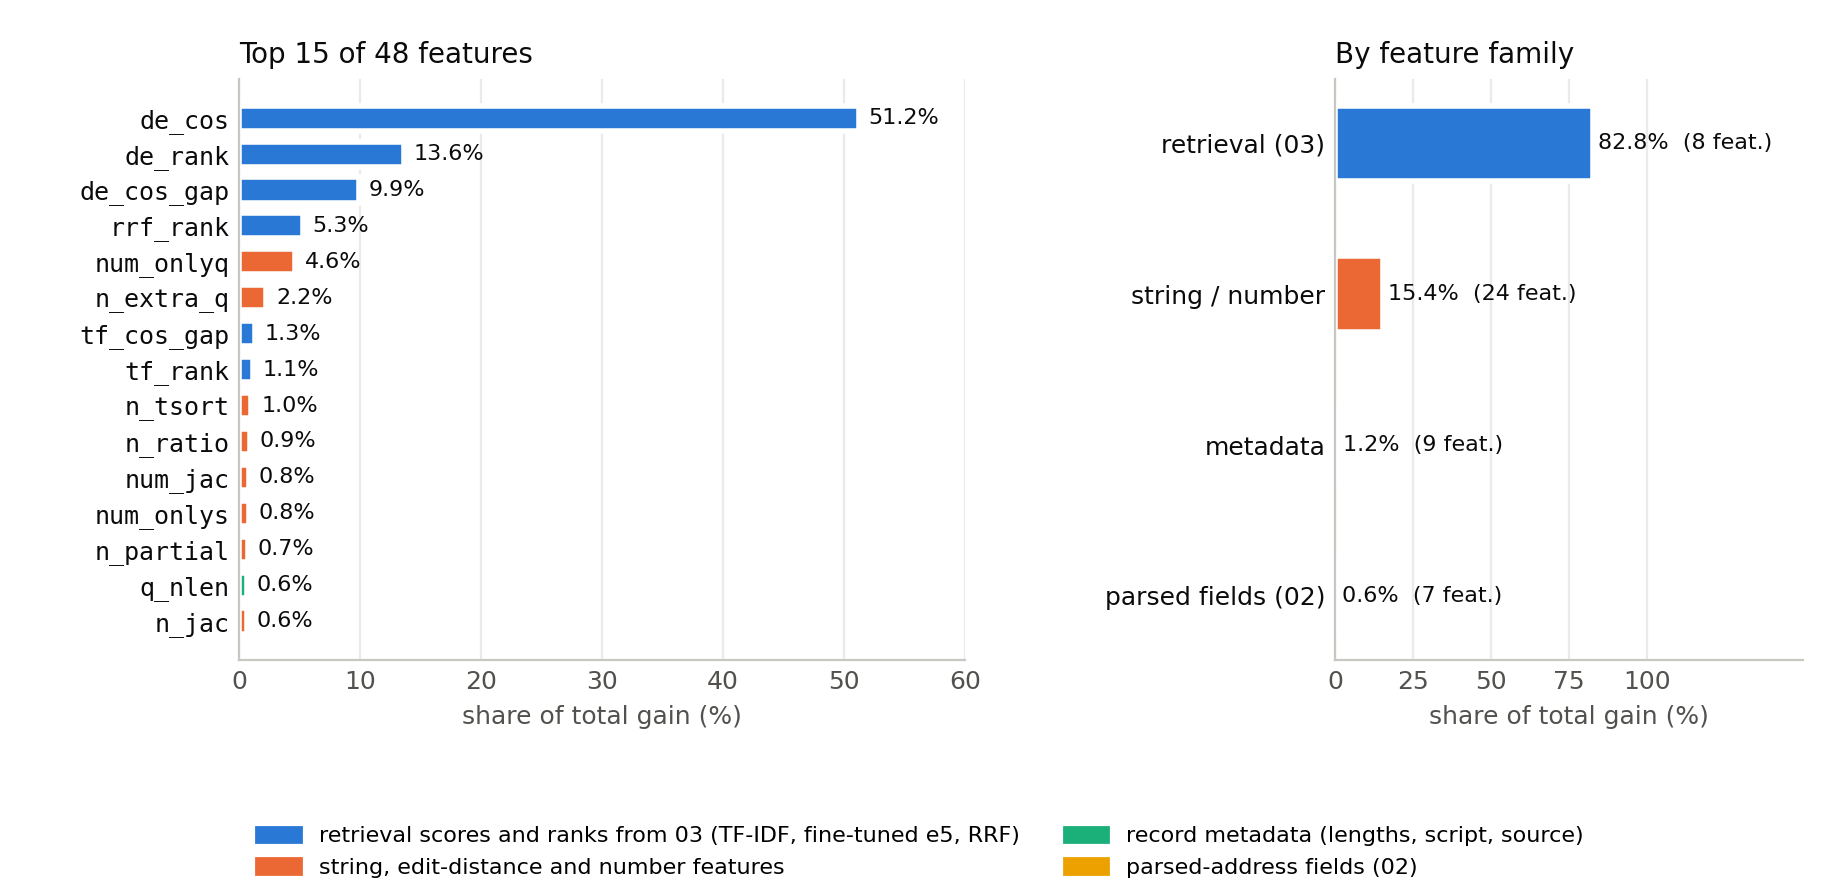
\includegraphics[width=0.92\linewidth]{gbm_feature_gain.png}
\caption{Share of the LightGBM split gain per feature (left, top 15 of 48) and per family (right).}
\label{fig:gbmgain}
\end{figure}

\paragraph{What the model uses.} Figure~\ref{fig:gbmgain} shows that \textbf{83\% of the gain comes from
\nb{03}'s retrieval features}. The fine-tuned e5 cosine alone has 51.2\%: it was trained on this task, and it
reads the original-script name, so it already captures matches that string ratios miss. Its rank (13.6\%)
and its gap to the best candidate (9.9\%) follow. The strongest hand-built feature is \texttt{num\_onlyq}
(4.6\%), the count of numbers in $q$'s address that do not appear in $s$. It is a hard negative signal: two
branches of a chain have near-identical names but different street numbers, and the embeddings blur exactly
that difference. String and number features together have 15.4\% of the gain (numbers 6.5\%), metadata
1.2\% and the parsed fields 0.6\%. So the GBM is a classical learner \emph{on top of a neural retriever}, not
a pure edit-distance model. We did not run it without the retrieval features.

\paragraph{Does the parser help matching?} We ran the GBM twice, once with BiLSTM-CRF fields and once with
rule fields. Test \fhalf{} is 0.99081 vs.\ 0.99051. A paired bootstrap over the 21,529 test
entities (10,000 resamples) gives a 95\% interval for the difference of
$[-0.00006, +0.00064]$. It includes 0, so the difference is \textbf{not significant}. The runs differ on only
273 entities (137 better with the BiLSTM-CRF, 136 with the rules). This is expected: with commas, both
parsers give the same fields for 99.7\% of addresses, and the parsed fields carry little gain. The parser's
advantage, comma-free addresses, does not occur in this data.

% Author: Rishi (condensed from report/section_recurrent_matchers.md)
\section{Recurrent matchers: Siamese character RNNs}
\label{sec:rnn}

\paragraph{Model.} The recurrent matchers read each record as a sequence of \emph{characters}, so typos,
abbreviations and transliteration variants (\emph{Glyfelle}/\emph{Glyphelle}) are small edits instead of
unknown words. The input is the normalised \texttt{name | address}, cut at 100 characters, over a vocabulary
of about 250 characters. A shared (Siamese) encoder embeds characters (64 dimensions), runs a bidirectional
recurrent layer (128 units per direction), and concatenates max- and mean-pooling over time into a record
vector $u\in\mathbb{R}^{512}$. For a record vector $u$ and a candidate vector $v$, an MLP scores
$[u; v; |u-v|; u\odot v]$~\citep{mueller2016siamese}. Three variants differ only in the cell: LSTM
(0.73M parameters), GRU (0.68M) and a vanilla Elman RNN (0.58M). They are trained with binary cross-entropy
on part-A candidate pairs, whose negatives are the hard ones retrieved by blocking: 3 epochs of 600k sampled
pairs, Adam, gradient clipping at norm 1.0.

\begin{table}[h]
\centering\small
\begin{tabular}{lccccccc}
\toprule
model & val \fhalf & test \fhalf & P & R & singleton acc. & params & train min \\
\midrule
Siamese char-BiLSTM (\nb{05a}) & 0.98920 & \textbf{0.98335} & 0.9863 & 0.9846 & 0.9454 & 0.73M & 13.3 \\
Siamese char-BiGRU (\nb{05b})  & 0.98814 & 0.98197 & 0.9850 & 0.9835 & 0.9404 & 0.68M & 13.1 \\
Siamese char-BiRNN (\nb{05c})  & 0.98374 & 0.97475 & 0.9782 & 0.9789 & 0.9085 & 0.58M & 11.9 \\
\bottomrule
\end{tabular}
\caption{Recurrent matchers on the test split (one T4 GPU).}
\label{tab:rnn}
\end{table}

\paragraph{Results.} The BiLSTM reaches 0.983 test \fhalf{} in 13 minutes, about 0.01 below the fine-tuned
cross-encoders with 380$\times$ fewer parameters (Table~\ref{tab:rnn}). LSTM and GRU differ by 0.0014, which
is within seed noise for single runs. The vanilla RNN loses 0.0086 against the BiLSTM, most of all on
singletons (0.909 vs.\ 0.945).

\begin{figure}[h]
\centering
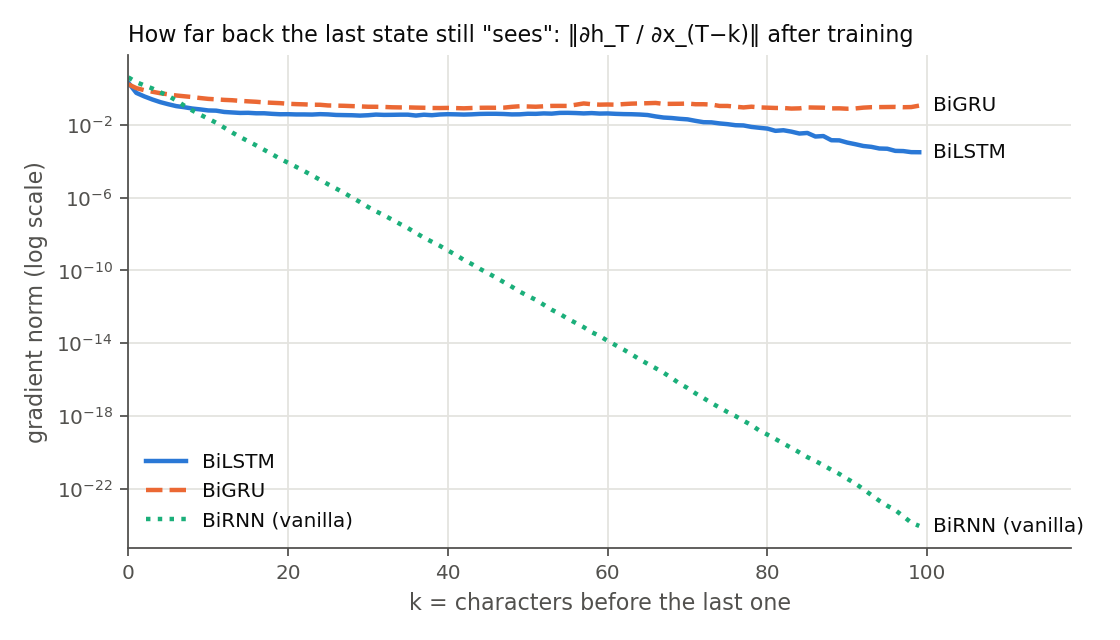
\includegraphics[width=0.72\linewidth]{rnn_grad_by_distance.png}
\caption{Gradient of the last forward state with respect to the input $k$ characters earlier, relative to
$k=0$, measured after training on 256 full-length training records.}
\label{fig:rnngrad}
\end{figure}

\paragraph{Why the vanilla RNN is worse: vanishing gradients, measured.} The vanilla RNN underfits: it has
the highest training loss at every epoch (0.044 vs.\ 0.029 for the LSTM after 3 epochs) and the largest
share of clipped steps (2.1\% in epoch 1). Figure~\ref{fig:rnngrad} measures its memory directly. For
$h_t=\tanh(Wh_{t-1}+Ux_t)$, the Jacobian $\partial h_T/\partial h_t=\prod_{s=t+1}^{T}\mathrm{diag}(1-h_s^2)\,W$
is a product of $T-t$ factors, and it shrinks geometrically~\citep{bengio1994learning,pascanu2013difficulty}:
by about 10$\times$ every 4 characters, reaching $10^{-12}$ at $k=50$. The LSTM and GRU carry state through
an additive, gated path ($\partial c_t/\partial c_{t-1}=\mathrm{diag}(f_t)$ for the LSTM), and after training
their gradient stays roughly flat over 100 characters ($2.0\times10^{-2}$ and $6.1\times10^{-2}$ at $k=50$).
At initialisation all three cells have tiny long-range gradients; only the gated cells \emph{learn} to open
the path. The gap is only about 0.01 because pooling over all time steps gives every character a short path
to the loss, and much matching evidence is local. What the vanilla RNN loses is evidence that spans the
string, such as a name token combined with a locality 60 characters later. That is what separates
near-duplicate branches, and it explains why singleton accuracy drops most.

\paragraph{Where they fail.} On the 283 records in other Indic scripts (Gujarati, Telugu, Tamil, \dots), all
three RNNs drop to 0.90--0.91, and every error is a missed link. They see only the romanised string, and
the generic romanisation of these scripts gives spellings far from the English S1 name
(\emph{emtrpraijes} for \emph{enterprises}) that the lexicon never learned (\S\ref{sec:script}).

% Authors: Shivam (06a, 06b, 06g Ditto), Keshav (06c LoRA, 06f mDeBERTa-v3), Ayush (06d MoE head),
% Rishi (06e IndicBERTv2).
% DRAFT by Keshav from the issue comments on #10, #11 and #20, because Shivam's section (#12) was not in yet.
% Replace or merge with Shivam's text if it arrives.
\section{Transformer cross-encoders}
\label{sec:ce}

\paragraph{Setup.} A cross-encoder reads the pair as one sequence, \texttt{[CLS]} $q$ \texttt{[SEP]} $s$, with both
records as \texttt{ce\_text} (original name, its romanisation, romanised address), and outputs a match
logit from the \texttt{[CLS]} vector~\citep{nogueira2019passage}. Every trained cross-encoder uses the same
recipe: one pass over 160,000 part-A candidate pairs (5,000 steps, batch 32, maximum length 96), binary
cross-entropy, and mixed precision (fp16 autocast) on one T4 GPU. Only the backbone, the learning rate and the
trained parameters change (Table~\ref{tab:ce}).

\begin{table}[h]
\centering\small
\resizebox{\linewidth}{!}{%
\begin{tabular}{llcccccc}
\toprule
 & model & trained params & test \fhalf & P & R & train min & peak GPU \\
\midrule
\nb{06a} & bge-reranker-base, zero-shot      & 0               & 0.91674 & 0.9161 & 0.9595 & 0    & 1.04 GB \\
\nb{06b} & bge-reranker-base, full fine-tune & 278M (100\%)    & 0.99124 & 0.9941 & 0.9878 & 19.4 & 5.53 GB \\
\nb{06c} & bge-reranker-base, LoRA $r{=}16$  & 1.48M (0.53\%)  & 0.98708 & 0.9900 & 0.9854 & 10.1 & 2.26 GB \\
\nb{06d} & bge-reranker-base + MoE head      & 279M (100\%)    & 0.98888 & 0.9914 & 0.9871 & 20.0 & -- \\
\nb{06e} & IndicBERTv2, full fine-tune       & 278M (100\%)    & 0.97611 & 0.9841 & 0.9666 & 19.3 & -- \\
\nb{06f} & mDeBERTa-v3-base, full, fp32      & 279M (100\%)    & \textbf{0.99402} & 0.9953 & 0.9931 & 60.4 & 9.31 GB \\
\bottomrule
\end{tabular}}
\caption{Cross-encoders on the test split. \nb{06a}--\nb{06d} share the backbone~\citep{xiao2023cpack}.}
\label{tab:ce}
\end{table}

\paragraph{Fine-tuning is what matters.} Without training, the reranker reaches 0.9167: high recall, low
precision, and only 0.687 accuracy on singletons, because it cannot tell a business from its near-duplicate
branches. Full fine-tuning adds \textbf{+0.0745} test \fhalf{} (0.9912), and singleton accuracy rises to 0.984.

\paragraph{LoRA.} LoRA~\citep{hu2022lora} freezes the backbone and trains rank-16 adapters on the query, key
and value projections of every layer (0.88M weights) plus the classification head (0.59M). With 0.53\% of the
weights it keeps \textbf{94\% of the fine-tuning gain} (0.98708). The 0.0042 gap to full fine-tuning is
consistent: full fine-tuning is ahead in every script group with enough records. LoRA needs 2.4$\times$ less
GPU memory and a 3\,MB instead of a 1.1\,GB checkpoint, but only 1.9$\times$ less training time, because the
forward and backward passes still run through the whole frozen backbone. On a 16\,GB T4, full fine-tuning
of this model fits anyway, so here LoRA is the cheaper option, not the necessary one.

\paragraph{mDeBERTa-v3 is the best single model} (0.9940), on both countries. It must train in fp32:
DeBERTa-v3 is unstable in fp16, and the T4 has no bf16. Our first run failed silently. The checkpoint is
stored in fp16, and our library version loads it in that dtype, so without autocast the whole model trained
in \emph{pure} fp16, with no fp32 master weights. Adam's $\epsilon=10^{-8}$ is 0 in fp16 and its small
second moments underflow. The loss was NaN from the first logged step, and the model predicted no matches
(\fhalf{} 0.055). Casting the weights to fp32 fixed it. The cost is 3.1$\times$ the training time of
\nb{06b} and 1.7$\times$ its memory.

\paragraph{MoE head (\nb{06d}).} The single classification head is replaced by four expert MLPs over the
\texttt{[CLS]} vector. A linear gate picks the top 2 per pair, with a Switch-style load-balancing
loss~\citep{shazeer2017outrageously,fedus2022switch} ($\lambda=0.01$). It scores 0.9889, slightly below plain
fine-tuning of the same backbone. Its experts do not specialise by script: their mean gate weights are almost
the same in every script ($\approx$0.21 / 0.22 / 0.23 / 0.33).

\paragraph{IndicBERTv2 (\nb{06e})} is the weakest fine-tuned cross-encoder (0.9761), even on Indic scripts;
\S\ref{sec:script} compares it with bge.

\paragraph{Ditto (\nb{06g}).} We reproduce Ditto~\citep{li2020ditto}:
\begin{itemize}
  \item records are serialised with attribute markers (\texttt{[COL] name [VAL] \dots});
  \item \textbf{DK} (domain knowledge) adds typed address spans from our parser (\S\ref{sec:parsing}) and
        normalised house numbers;
  \item \textbf{SU} (summarisation) keeps the highest-TF-IDF tokens instead of truncating;
  \item \textbf{DA} interpolates the encodings of a pair and an augmented copy (MixDA).
\end{itemize}
The backbone is xlm-roberta-base, except R6, which starts from bge-reranker-base. Each run uses 40k
training pairs and one seed. The ablation was run twice, with rule-parsed and with BiLSTM-CRF-parsed spans
(Table~\ref{tab:ditto}).

\begin{table}[h]
\centering\small
\begin{tabular}{llcc}
\toprule
run & backbone & test \fhalf, rule spans & test \fhalf, BiLSTM-CRF spans \\
\midrule
R1 plain           & XLM-R & 0.9788 & 0.9782 \\
R2 +DK             & XLM-R & 0.9803 & 0.9823 \\
R3 +SU             & XLM-R & 0.9754 & 0.9774 \\
R4 +DA             & XLM-R & 0.9817 & 0.9761 \\
R5 +DK+SU+DA       & XLM-R & 0.9779 & 0.9798 \\
R6 +DK+SU+DA       & bge   & \textbf{0.9821} & \textbf{0.9828} \\
\bottomrule
\end{tabular}
\caption{Ditto ablation, 40k training pairs per run. Table~\ref{tab:main} uses the rule-span runs.}
\label{tab:ditto}
\end{table}

R1, R3 and R4 do not use the parser, so their configurations are identical in both runs. They still
differ by up to 0.0056 (R4), and DA even changes sign against R1 (+0.0029, then $-0.0021$). Run-to-run
noise is therefore up to about 0.006. DK is the only optimisation that is positive in both runs, and more
so with our parser (+0.0015 and +0.0041 over R1), but even this is within the noise. With a quarter of the training pairs, the best Ditto run
(0.9828) stays below \nb{06b} (0.9912). The full-size Ditto run, which would make the two comparable, was not
completed.

% Author: Ayush (condensed from demo/report_section_moe_results.md); main table from final_results.md
\section{Gated Mixture-of-Experts fusion and main results}
\label{sec:fusion}

\paragraph{Model.} The fusion treats each matcher as an expert. For a candidate
pair with expert logits $z_1,\dots,z_N$ (z-scored on part B) and gate features $x$, it predicts
\[
p=\sigma\Big(\sum_{i=1}^{N} w_i(x)\,(a_i z_i+b_i)+c\Big),\qquad w(x)=\mathrm{softmax}\big(W_2\,\mathrm{ReLU}(W_1x)\big),
\]
with a per-expert affine calibration $(a_i,b_i)$, initialised from one logistic fit per expert, so training
starts at the mean of calibrated experts. The gate is an MLP with 32 hidden units over 13 features of the
record and its retrieval:
\begin{itemize}
  \item script (4 indicators), source S3, empty address, address contains a number;
  \item name and address length;
  \item TF-IDF and e5 cosines, RRF rank, number of candidates.
\end{itemize}
It never sees the country. The fusion is trained on the part-B pairs that no expert was trained on, with
binary cross-entropy (Adam, learning rate $10^{-2}$, batch 2048, cosine schedule). The nine experts are
\nb{04}, \nb{05a}, \nb{05b} and \nb{06a}--\nb{06f}. We compare it with four alternatives:
\begin{itemize}
  \item the mean of the calibrated experts;
  \item logistic-regression stacking on the logits;
  \item LightGBM stacking on the logits plus the gate features;
  \item the same MoE with a \emph{constant} gate, i.e.\ learned weights that do not depend on $x$.
\end{itemize}

\begin{table}[t]
\centering\small
\resizebox{\linewidth}{!}{%
\begin{tabular}{llcccccccc}
\toprule
 & method & val \fhalf & test \fhalf & P & R & US & India & single. & min \\
\midrule
\multirow{1}{*}{classical}
 & LightGBM (\nb{04})                  & 0.99286 & 0.99081 & 0.9938 & 0.9873 & 0.98946 & 0.99205 & 0.9857 & 4.6 \\
\midrule
\multirow{3}{*}{RNN}
 & Siamese char-BiLSTM (\nb{05a})       & 0.98920 & 0.98335 & 0.9863 & 0.9846 & 0.98390 & 0.98284 & 0.9454 & 13.3 \\
 & Siamese char-BiGRU (\nb{05b})        & 0.98814 & 0.98197 & 0.9850 & 0.9835 & 0.98142 & 0.98247 & 0.9404 & 13.1 \\
 & Siamese char-BiRNN (\nb{05c})        & 0.98374 & 0.97475 & 0.9782 & 0.9789 & 0.97646 & 0.97316 & 0.9085 & 11.9 \\
\midrule
\multirow{8}{*}{transformer}
 & mDeBERTa-v3 full FT, fp32 (\nb{06f}) & 0.99561 & \textbf{0.99402} & 0.9953 & 0.9931 & 0.99261 & 0.99533 & 0.9866 & 60.4 \\
 & bge full FT (\nb{06b})               & 0.99338 & 0.99124 & 0.9941 & 0.9878 & 0.98935 & 0.99299 & 0.9840 & 19.4 \\
 & bge + MoE head (\nb{06d})            & 0.99226 & 0.98888 & 0.9914 & 0.9871 & 0.98719 & 0.99044 & 0.9706 & 20.0 \\
 & bge LoRA $r{=}16$ (\nb{06c})         & 0.99142 & 0.98708 & 0.9900 & 0.9854 & 0.98566 & 0.98839 & 0.9681 & 10.1 \\
 & Ditto final, XLM-R DK+SU+DA, 160k (\nb{06g}) & 0.98998 & 0.98758 & 0.9923 & 0.9805 & 0.98822 & 0.98699 & 0.9757 & 29.3 \\
 & Ditto, bge DK+SU+DA, 40k (\nb{06g})  & 0.98713 & 0.98214 & 0.9856 & 0.9813 & 0.98158 & 0.98266 & 0.9379 & 7.5 \\
 & IndicBERTv2 full FT (\nb{06e})       & 0.98249 & 0.97611 & 0.9841 & 0.9666 & 0.97268 & 0.97929 & 0.9446 & 19.3 \\
 & bge zero-shot (\nb{06a})             & 0.94192 & 0.91674 & 0.9161 & 0.9595 & 0.92713 & 0.90712 & 0.6868 & 0 \\
\midrule
\multirow{5}{*}{fusion}
 & \textbf{Gated MoE} (\nb{07})         & 0.99648 & \textbf{0.99481} & 0.9961 & 0.9935 & 0.99304 & 0.99645 & 0.9933 & 0.17 \\
 & Logistic-regression stacking         & 0.99648 & 0.99477 & 0.9967 & 0.9920 & 0.99322 & 0.99620 & 0.9933 & \\
 & MoE, constant gate (ablation)        & 0.99642 & 0.99474 & 0.9963 & 0.9928 & 0.99299 & 0.99636 & 0.9933 & \\
 & LightGBM stacking                    & 0.99632 & 0.99470 & 0.9968 & 0.9918 & 0.99305 & 0.99622 & 0.9924 & \\
 & Mean of 9 calibrated experts         & 0.99525 & 0.99286 & 0.9941 & 0.9927 & 0.99204 & 0.99363 & 0.9857 & \\
\midrule
 & blocking ceiling (perfect matcher)   &         & 0.99957 & & & & & & \\
\bottomrule
\end{tabular}}
\caption{Main results. Macro \fhalf{} on val and test, test precision and recall, test \fhalf{} per
country, singleton accuracy and training minutes. Thresholds are tuned on val, and test is scored once.
Ditto rows were run after the fusion experts were fixed, so the gated MoE does not include them. The other Ditto runs are in Table~\ref{tab:ditto}.}
\label{tab:main}
\end{table}

\paragraph{Results.} The gated MoE reaches \textbf{0.99481} test \fhalf{} (Table~\ref{tab:main}). It is
+0.0008 above the best single model, mDeBERTa-v3, a gain that is significant in a paired bootstrap over test
entities, and +0.0020 above the mean of the experts. Every fusion except the plain mean lies within
0.0002 of it. The constant-gate ablation reaches 0.99474, and its gap to the gated MoE (+0.00007) is not
significant. \textbf{The gain therefore comes from learned, calibrated weights over complementary experts,
not from routing each pair by its properties.}

\begin{table}[h]
\centering\small
\begin{tabular}{lccc}
\toprule
script of the S2/S3 record & LightGBM & mDeBERTa-v3 & other 7 experts \\
\midrule
Latin       & 0.60 & 0.36 & 0.03 \\
Devanagari  & 0.74 & 0.23 & 0.03 \\
Malayalam   & 0.75 & 0.24 & 0.01 \\
other Indic & 0.91 & 0.09 & 0.01 \\
\bottomrule
\end{tabular}
\caption{Mean gate weight per expert on test, by script.}
\label{tab:gate}
\end{table}

\paragraph{What the gate learns.} The fusion is essentially a two-expert blend (Table~\ref{tab:gate}):
LightGBM gets 60--91\% of the weight, mDeBERTa-v3 the rest, and every other expert, IndicBERTv2 included,
gets under 2\% each. These two are the most \emph{different} experts. The GBM decides from retrieval scores
and explicit number and word mismatches, mDeBERTa from reading both records jointly. The other
cross-encoders read the records the same way mDeBERTa does and add little on top of it. The weight moves
toward the GBM on Indic scripts, whose strongest feature, the e5 similarity, is computed on the
original-script name.

% Author: Rishi (condensed from report/section_script_analysis.md)
\section{Per-script analysis}
\label{sec:script}

All S1 records are in Latin script; the S2/S3 records come in several scripts. We group every test S2/S3
record by country $\times$ script: US Latin (48,710 records), India Latin (34,342), Devanagari (7,868),
Malayalam (10,371), and other Indic scripts (283; Gujarati, Telugu, Tamil, Kannada, Bengali, Odia,
Gurmukhi). About half of the Devanagari and Malayalam records have the business name itself in that script.
Macro \fhalf{} is computed per group from each model's unchanged predictions (Table~\ref{tab:script}).

\begin{table}[h]
\centering\small
\begin{tabular}{lccccc}
\toprule
model & US Latin & India Latin & Devanagari & Malayalam & other Indic (283) \\
\midrule
LightGBM (\nb{04})            & 0.9889 & 0.9860 & 0.9924 & 0.9909 & 1.0000 \\
Siamese BiLSTM (\nb{05a})     & 0.9830 & 0.9754 & 0.9831 & 0.9781 & 0.9048 \\
bge zero-shot (\nb{06a})      & 0.9242 & 0.8944 & 0.8826 & 0.8857 & 0.9615 \\
bge full FT (\nb{06b})        & 0.9887 & 0.9878 & 0.9935 & 0.9915 & 0.9441 \\
IndicBERTv2 full FT (\nb{06e})& 0.9712 & 0.9684 & 0.9728 & 0.9778 & 0.9715 \\
mDeBERTa-v3 full FT (\nb{06f})& 0.9922 & 0.9901 & 0.9969 & 0.9970 & 0.9815 \\
Gated MoE (\nb{07})           & 0.9926 & 0.9922 & 0.9964 & 0.9975 & 0.9975 \\
\bottomrule
\end{tabular}
\caption{Test \fhalf{} per script group (selected models; all 21 in \texttt{analysis/out\_script/}).}
\label{tab:script}
\end{table}

\paragraph{Script is not what makes a record hard.} For almost every trained model, India Latin is the
hardest of the four main groups. That holds for all five fusion models too, and every fully fine-tuned
cross-encoder scores \emph{higher} on Devanagari and Malayalam than on either Latin group. Fine-tuning is
what closes the script gap: zero-shot bge is the one model that is weakest on native scripts (0.883 on
Devanagari), and full fine-tuning lifts the same backbone to 0.994 (+0.11). The difficulty lies in the records
themselves: near-duplicate branches, missing addresses and generic names.

\paragraph{Romanised-only models fail on rare scripts.} On the 283 other-Indic records, the char-RNNs drop to
0.90--0.91, while the cross-encoders, which also read the original-script name, stay at 0.94--0.98. The GBM
reaches 1.000 there. Its strongest feature, the e5 cosine, is also computed on the original-script name, but
283 records (17 unlinked) are too few for strong claims.

\paragraph{The Indic-specific backbone loses.} IndicBERTv2 and bge-reranker-base were fine-tuned with the
same recipe. On the Indian records, bge is significantly better on Latin, Devanagari and Malayalam, in both
\fhalf{} and threshold-free AUC. An exact McNemar test on the records that only one
model gets right gives $p\le 6\times10^{-18}$; on Devanagari, for example, 139 records are right only with
bge and 27 only with IndicBERTv2. On the 283 other-Indic records the two tie (7 vs.\ 6 records). We see two
likely reasons:
\begin{itemize}
  \item bge-reranker was already pre-trained as a cross-encoder for relevance, while IndicBERTv2 is an
        MLM-only encoder whose pairwise head starts from scratch;
  \item the decisive tokens (names, house numbers, localities) are mostly Latin or romanised on at least
        one side, since S1 is always Latin.
\end{itemize}
The ranking of the cross-encoders (mDeBERTa-v3 $>$ bge full $>$ MoE head $>$ LoRA $>$ IndicBERTv2 $>$
zero-shot) is the same in every main script group.

\paragraph{Errors are shared and data-driven.} Blocking misses are the same for every model (96 test records)
and are a small share of each model's errors. Pair AUC is at least 0.998 for every fine-tuned model in every
main group, so most remaining errors come from the decision on near-duplicates. Some errors are made by
almost every model, fusion included:
\begin{itemize}
  \item a business whose house number differs from its S1 neighbour's by 4, which models read as a typo;
  \item two S1 branches with the same name and an S2 record without an address, so nothing can choose
        between them;
  \item mixed-script records that retrieval never paired with their S1.
\end{itemize}
The script-specific errors, such as a Kannada name that matches only after transliteration, belong to a few
single models, and the fusion fixes them. Against mDeBERTa-v3, the gated MoE gains most on India Latin
(+0.002) and the other Indic records (+0.016, 2 errors instead of 7).

% Author: Keshav
\section{Conclusion}
\label{sec:conclusion}

We built a shared pipeline for multilingual business entity resolution and compared matchers from three
model families on identical candidate pairs. Five results stand out.
\begin{enumerate}
  \item \textbf{Task fine-tuning matters more than the backbone.} It lifts the bge cross-encoder from 0.9167
        to 0.9912, and it closes the script gap. LoRA keeps 94\% of that gain with 0.53\% of the weights.
  \item \textbf{Retrieval carries more than it seems.} The candidate generator leaves almost no recall on the
        table (ceiling 0.99957). Its fine-tuned e5 similarity is also the main input of the classical
        LightGBM (83\% of the gain), which comes within 0.0004 of a fully fine-tuned cross-encoder in under
        5 CPU minutes.
  \item \textbf{Gated recurrence matters, and we can measure why.} LSTM and GRU beat a vanilla RNN by about
        0.009. After training, the vanilla RNN's dependence on a character 50 positions back is $10^{-12}$.
  \item \textbf{Language coverage is not pairwise skill.} IndicBERTv2 tokenizes Indic text best but matches
        worst among the fine-tuned cross-encoders, even on Indic scripts.
  \item \textbf{Fusion helps through complementarity, not routing.} The gated MoE (0.9948) beats every single
        matcher, but a constant gate does as well. The useful structure is a blend of the classical model
        and the best cross-encoder.
\end{enumerate}

\paragraph{Limitations.}
\begin{itemize}
  \item Our splits have about half the official distractor density and 3.5\% of the entities, so the
        absolute scores are optimistic.
  \item Most comparisons rest on a single seed, and the 06g reruns show run-to-run noise of up to 0.006.
  \item The parser is trained and evaluated on silver labels.
  \item We did not run the GBM without its retrieval features, so the strength of a purely string-based
        model on this data is open.
  \item The 160k-pair Ditto run used the XLM-R backbone (0.9876); a bge-based one, the best at 40k, was not run.
\end{itemize}

\paragraph{Contributions.}
\begin{center}\small
\begin{tabularx}{\linewidth}{lX}
\toprule
member & work \\
\midrule
Akshat & data splits and metric, tokenization study (\nb{01}), candidate generation (\nb{03}), shared Kaggle datasets, slide deck \\
Keshav & address parser (\nb{02}), LightGBM baseline (\nb{04}), LoRA and mDeBERTa-v3 cross-encoders (\nb{06c}, \nb{06f}), report assembly \\
Rishi  & Siamese RNNs (\nb{05a}--\nb{c}), IndicBERTv2 cross-encoder (\nb{06e}), per-script error analysis \\
Shivam & bge zero-shot and full fine-tuning (\nb{06a}, \nb{06b}), Ditto (\nb{06g}), README results \\
Ayush  & MoE head (\nb{06d}), gated MoE fusion and results (\nb{07}), live demo (\nb{08}) \\
\bottomrule
\end{tabularx}
\end{center}
Code, notebooks and the full analyses behind every section are in the project repository.


\end{document}
